% \section{The advantages of combining resolution and precision}
% \label{sec:motivation}

% Traditional data reduction techniques work by truncating either the finest few resolution levels, or
% the last few low-ordered bits, but rarely both. In this section, we show that significant gain can
% be achieved through reducing both data resolution and precision. For each data set, we construct and
% compare four different streams, namely \emph{by level}, \emph{by bit plane}, \emph{by wavelet norm},
% and \emph{by magnitude}. The first three streams were introduced in
% Section~\ref{sec:common-static-streams}. The \emph{by magnitude} stream mimics a common data
% reduction scheme in the literature, in which the smaller-magnitude wavelet coefficients are removed.
% Correspondingly, in \emph{by magnitude}, the chunks are sorted by the sum of magnitude of their
% respective coefficients, and chunks of the same coefficient are streamed together. 

% We compare the four streams using three common quantities, namely the function itself, the
% function's histogram, and an isocontour. Every time a new chunk arrives, we reconstruct the function
% (using the inverse wavelet transform) on the original-resolution grid, and compute the
% root-mean-square error between this reconstructed function and the original function. For the other
% two quantities, the RMSE is replaced by relevant error metrics (see Section~\ref{sec:histogram}
% and~\ref{sec:isocontour} for detailed discussions of these error metrics).
% Figure~\ref{fig:motivation-rmse} shows the results. Note that in all plots, we remove all chunks
% containing purely leading zero bits, as such chunks tend to be compressed away in practice. 

% \begin{figure}[h]
%   \centering
% 	\subcaptionbox{RMSE, left: \emph{plasma}, right: \emph{turbulence}}{
%   {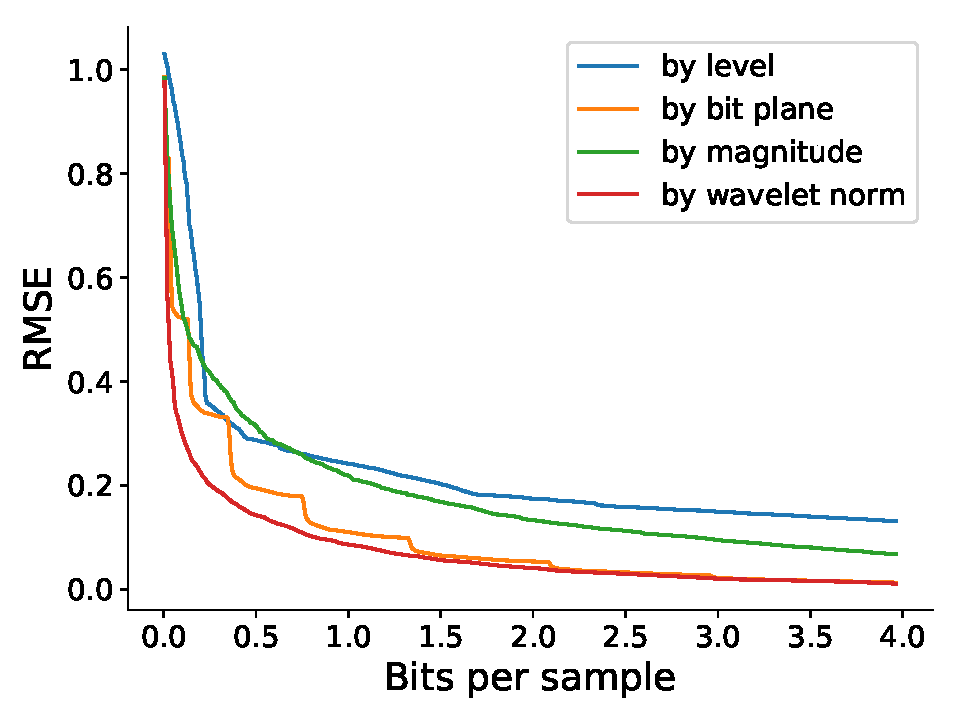
\includegraphics[width=0.48\linewidth]{img/motivation/motivation-psnr-plasma.pdf}}
%   {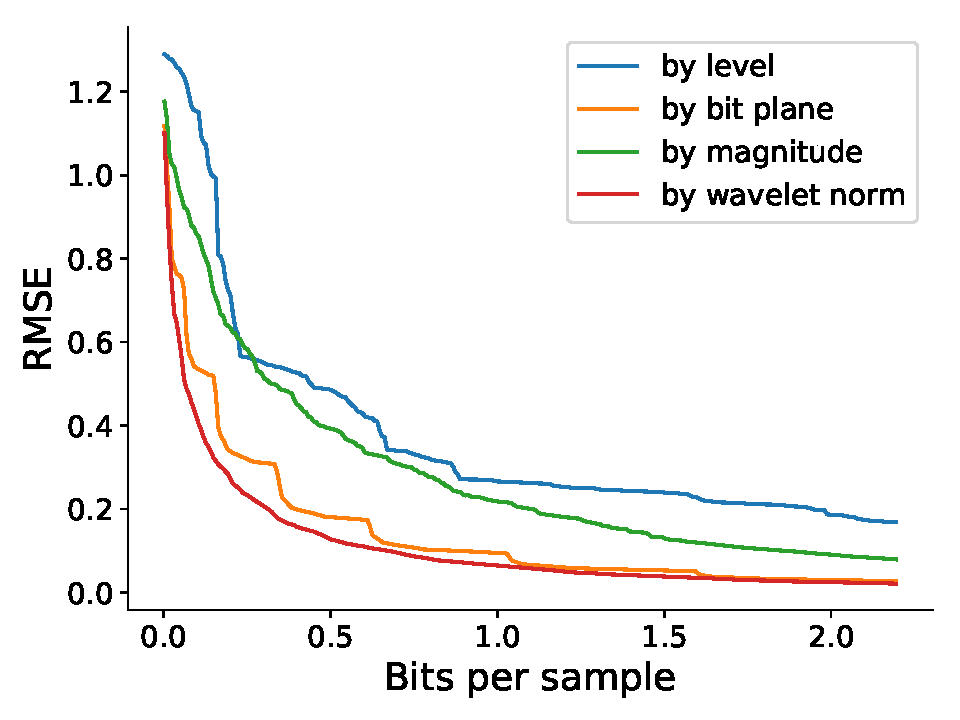
\includegraphics[width=0.48\linewidth]{img/motivation/motivation-psnr-turbulence.pdf}}}
%   \subcaptionbox{Histogram, left: \emph{plasma}, right: \emph{turbulence}}{
%   {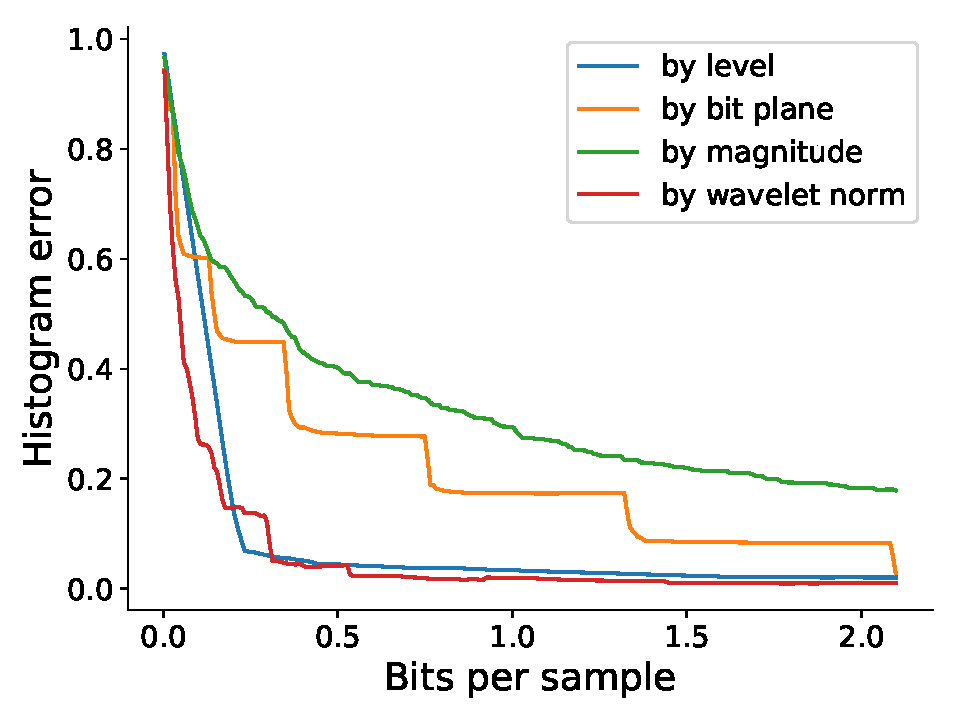
\includegraphics[width=0.48\linewidth]{img/motivation/motivation-histogram-plasma.pdf}}
%   {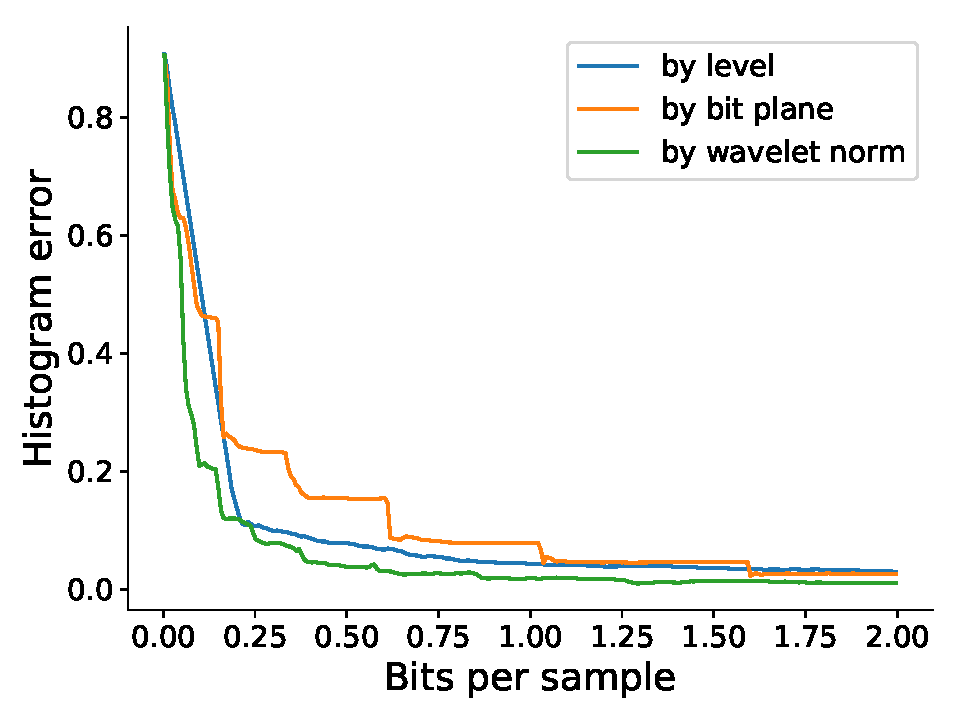
\includegraphics[width=0.48\linewidth]{img/motivation/motivation-histogram-turbulence.pdf}}}
%   \subcaptionbox{Isocontour, left: \emph{plasma}, right: \emph{turbulence}}{
%   {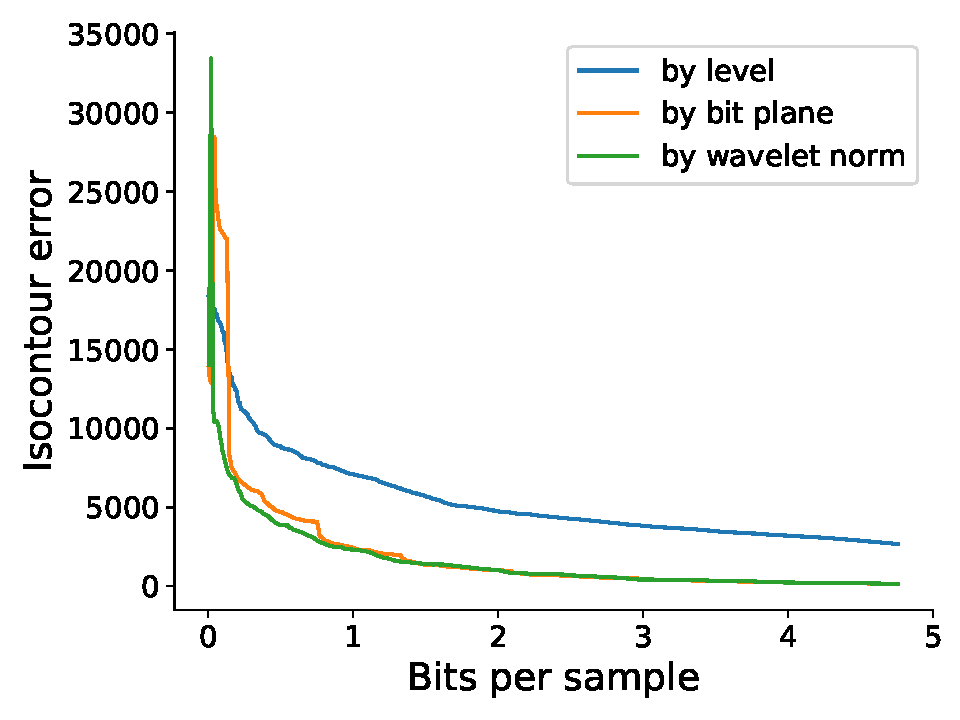
\includegraphics[width=0.48\linewidth]{img/motivation/motivation-isocontour-plasma.pdf}}
%   {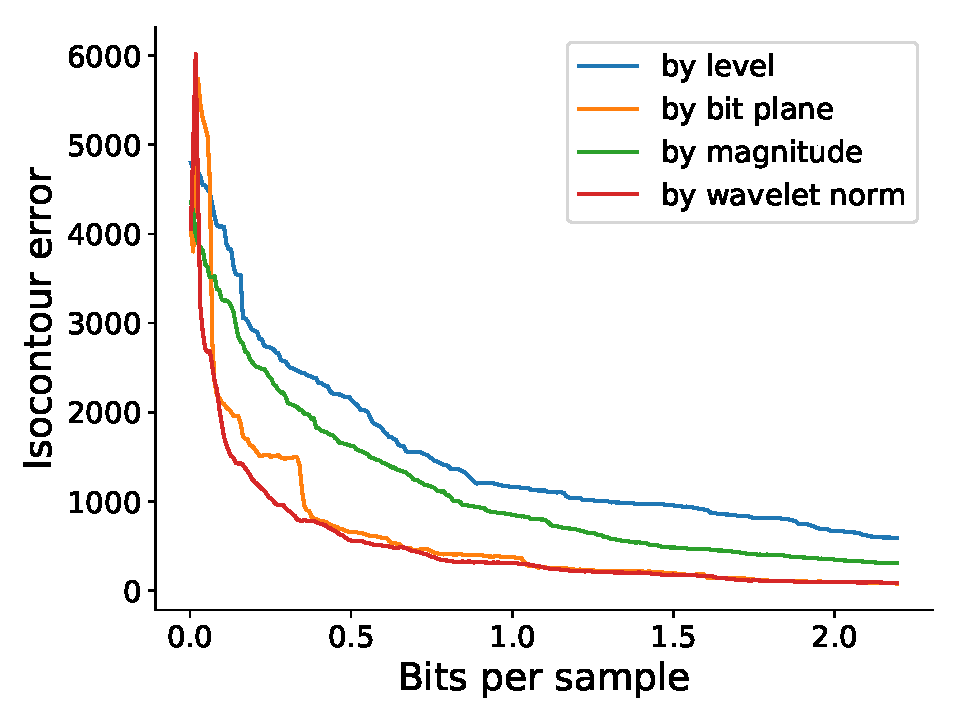
\includegraphics[width=0.48\linewidth]{img/motivation/motivation-isocontour-turbulence.pdf}}}
%   \caption{Comaprisons of the three static streams defined in Section \ref{sec:motivation}. Lower
%   error is better. The plots are truncated to better highlight the differences, without omitting
%   important information. Chunks containing leading zero bits are not plotted. In all cases, \emph{by
%   wavelet norm} performs the best.}
%  	\label{fig:motivation-rmse}
% \end{figure}

% The \emph{by wavelet norm} stream can be seen to consistently performs the best, across all data
% sets and quantities of interest. \emph{by bit plane} works almost as well as \emph{by wavelet norm}
% for function reconstruction and isocontour extraction, but not for histogram computation. The
% reverse is true for \emph{by level}. The \emph{by magnitude} stream performs somewhat better than
% \emph{by level}, except for histogram computation. Note that the our removal of leading zero bits
% penalizes the \emph{by level} stream more than it does the other streams, because in a typical data
% set, most leading-zero chunks exist in fine-resolution subbands (i.e., fine-scale coefficients tend
% to be smaller), which \emph{by level} only accesses later in the stream. The reason \emph{by wavelet
% norm} performs better than the rest is that a higher-ordered bit from a fine-scale coefficient might
% contribute more than a lower-ordered bit from a coarse-scale coefficient does (which \emph{by
% levell} is unable to take advantage of), and vice-versa (which \emph{by bit plane} ignores).

% The fact that \emph{by wavelet norm} outperforms all the other three suggests that performing data
% reduction in both resolution and precision can lead to significant quality improvements. In
% addition, it is possible that different analysis tasks require different types of streams for
% optimal results. This is hinted at by the fact that \emph{by level} underperforms \emph{by bit
% plane} for two of the three tasks, but outperforms it for the third (histogram). It seems likely,
% but uncertain at this point, whether \emph{by wavelet norm} is the best in all cases. To answer this
% question, we will expand our study to include dynamic streams that are optimized specifically for
% each quantity. While these data-dependent streams are unlikely to be realizable in practice, they
% can provide insights into designing practical data streams that improve on the generic \emph{by
% wavelet norm}, by being tailored to the analysis task at hand.
